\section{Use cases}



\begin{figure}[H]
\centering
  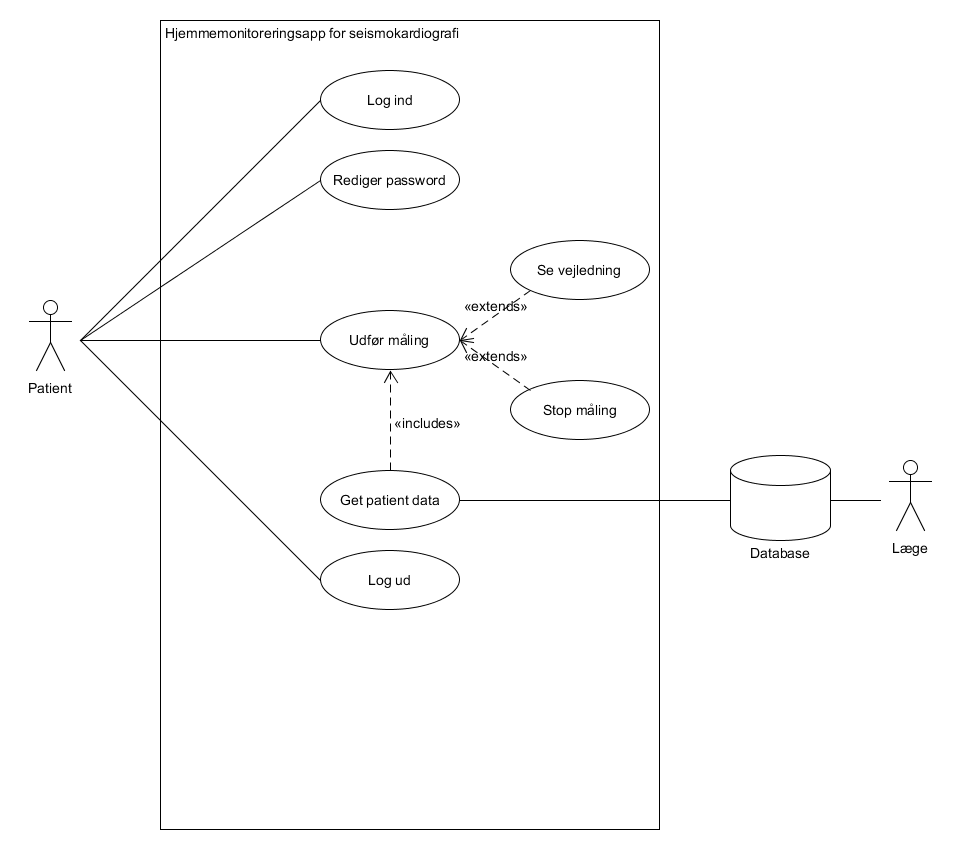
\includegraphics[width=1.1\textwidth]{Billeder/app}
   \caption{Overordnet use case diagram} 
   \label{...}
\end{figure}

\begin{figure}[H]
\centering
  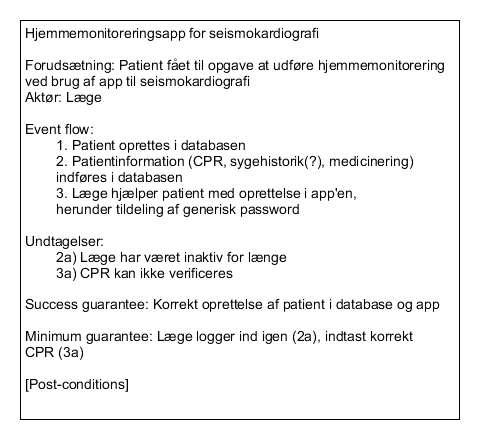
\includegraphics[width=0.6\textwidth]{Billeder/oprettelse.png}
   \caption{Udvidet use case oprettelse} 
   \label{fig:hjerte}
\end{figure}


\begin{figure}[H]
\centering
  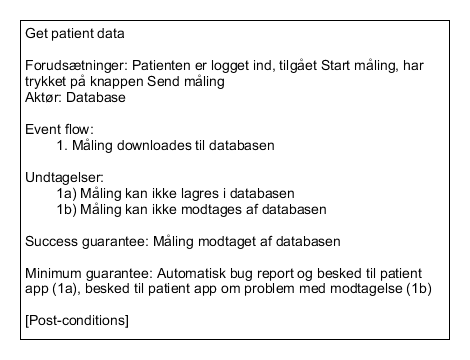
\includegraphics[width=0.6\textwidth]{Billeder/getpatient.png}
   \caption{Udvidet use case for get patient} 
   \label{fig:hjerte}
\end{figure}




\begin{figure}[H]
\centering
  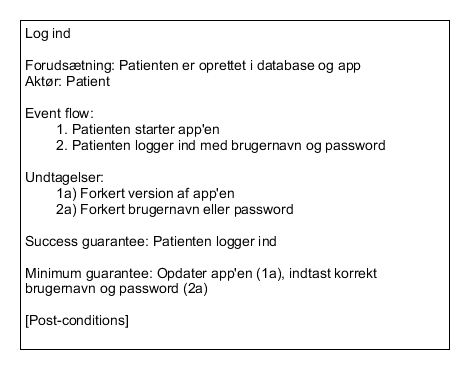
\includegraphics[width=0.6\textwidth]{Billeder/logind}
   \caption{Udvidet use case for log ind} 
   \label{fig:hjerte}
\end{figure}



\begin{figure}[H]
\centering
  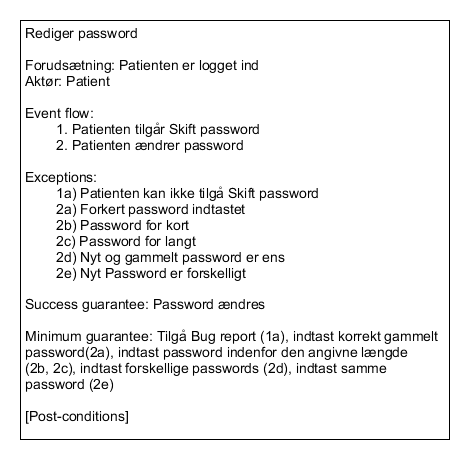
\includegraphics[width=0.6\textwidth]{Billeder/redpass.png}
   \caption{Udvidet use case for rediger password} 
   \label{fig:hjerte}
\end{figure}


\begin{figure}[H]
\centering
  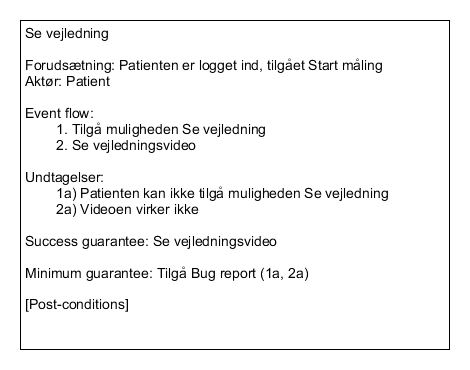
\includegraphics[width=0.6\textwidth]{Billeder/sevejledning.png}
   \caption{Use case se vejledning} 
   \label{fig:hjerte}
\end{figure}


\begin{figure}[H]
\centering
  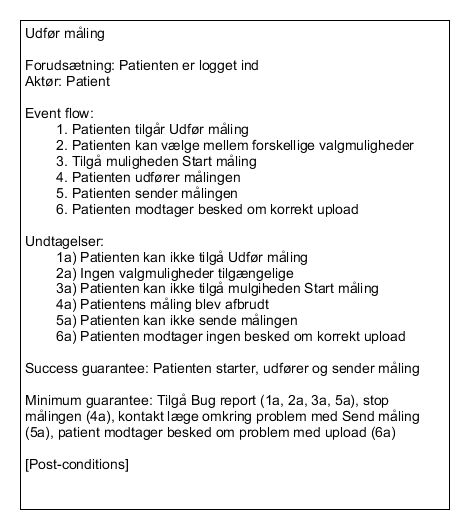
\includegraphics[width=0.6\textwidth]{Billeder/startmaling.png}
   \caption{Use case udvidet start måling} 
   \label{fig:hjerte}
\end{figure}


\begin{figure}[H]
\centering
  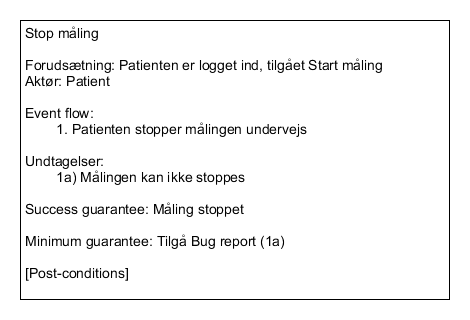
\includegraphics[width=0.6\textwidth]{Billeder/stopmaling.png}
   \caption{Udvidet use case for stop måling} 
   \label{fig:hjerte}
\end{figure}




\begin{figure}[H]
\centering
  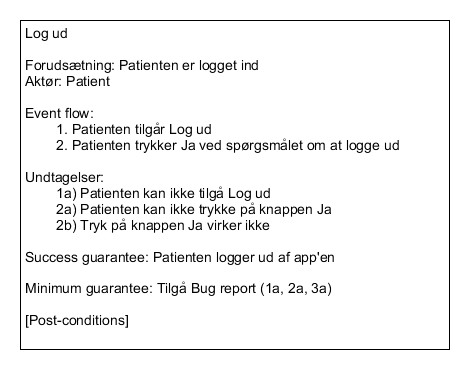
\includegraphics[width=0.6\textwidth]{Billeder/logud.png}
   \caption{Udvidet use case for log ud} 
   \label{fig:hjerte}
\end{figure}


\begin{figure}[H]
\centering
  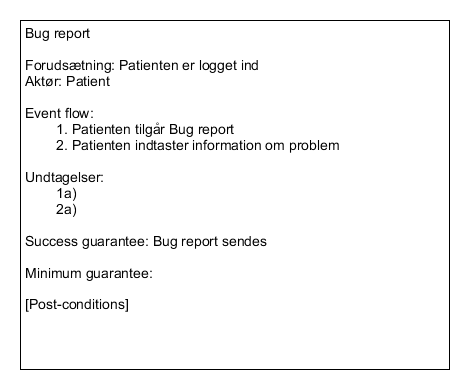
\includegraphics[width=0.6\textwidth]{Billeder/bugreport.png}
   \caption{Udvidet use case for bug report} 
   \label{fig:hjerte}
\end{figure}


%%%%%%%%%%%%%5
\begin{table}[H]
\centering
\label{useudformaling}
\begin{tabular}{|l|}
\hline
\multicolumn{1}{|c|}{\textbf{Use case 'udfør måling'}}                                     \\ \hline
\begin{tabular}[c]{@{}l@{}}\textbf{Aktør}\\ Bruger\end{tabular}                              \\ \hline
\begin{tabular}[c]{@{}l@{}}\textbf{Forudsætninger}\\ Bruger er oprettet i systemet og logget ind\end{tabular}                       \\ \hline
\begin{tabular}[c]{@{}l@{}}\textbf{Triggers}\\ Knappen 'Udfør måling' trykkes\end{tabular}                             \\ \hline
\begin{tabular}[c]{@{}l@{}}\textbf{Success scenarie}\\     1. Bruger tilgår 'Udfør måling'\\     2. Bruger vælger valgmuligheden 'Start måling'\\     3. Bruger udfører måling\end{tabular}       \\ \hline
\begin{tabular}[c]{@{}l@{}}\textbf{Følgetilstand}\\ Bruger starter og udfører måling\end{tabular}                       \\ \hline 
\begin{tabular}[c]{@{}l@{}}\textbf{Alternativt scenarie}\\     1a) Bruger kan ikke tilgå 'Udfør måling'\\ - Returner fejlmeddelelse\\  2a) Ingen valgmuligheder tilgængelige\\     2b) Bruger kan ikke tilgå valgmuligheden 'Start måling'\\     3a) Bruger kan ikke udføre måling\end{tabular} \\ \hline
\end{tabular}
\caption{Udvidet use case for 'Udfør måling'}
\end{table}

\begin{table}[H]
\centering
\label{usesevejledning}
\begin{tabular}{|l|}
\hline
\multicolumn{1}{|c|}{\textbf{Use case 'se vejledning'}}                                     \\ \hline
\begin{tabular}[c]{@{}l@{}}\textbf{Aktør}\\ Bruger\end{tabular}                              \\ \hline
\begin{tabular}[c]{@{}l@{}}\textbf{Forudsætninger}\\ Bruger er tilgået 'Udfør måling'\end{tabular}                       \\ \hline
\begin{tabular}[c]{@{}l@{}}\textbf{Triggers}\\ Knappen 'Se vejledning' trykkes\end{tabular}                             \\ \hline
\begin{tabular}[c]{@{}l@{}}\textbf{Success scenarie}\\     1. Bruger tilgår valgmuligheden 'Se vejledning'\\     2. Bruger ser vejledningsvideo\end{tabular}       \\ \hline
\begin{tabular}[c]{@{}l@{}}\textbf{Følgetilstande}\\ Bruger ser vejledningsvideo\end{tabular}                       \\ \hline
\begin{tabular}[c]{@{}l@{}}\textbf{Alternativt scenarie}\\     1a) Bruger kan ikke tilgå valgmuligheden 'Se vejledning'\\     2a) Vejledningsvideoen virker ikke\end{tabular} \\ \hline
\end{tabular}
\caption{Udvidet use case for 'Se vejledning'}
\end{table}


\begin{table}[H]
\centering
\label{usestopmaling}
\begin{tabular}{|l|}
\hline
\multicolumn{1}{|c|}{\textbf{Stop måling}}                                     \\ \hline
\begin{tabular}[c]{@{}l@{}}\textbf{Aktører}\\ Bruger\end{tabular}                              \\ \hline
\begin{tabular}[c]{@{}l@{}}\textbf{Forudsætninger}\\ Bruger er tilgået valgmuligheden Start måling\end{tabular}                       \\ \hline
\begin{tabular}[c]{@{}l@{}}\textbf{Triggers}\\ Knappen Stop måling trykkes\end{tabular}                             \\ \hline
\begin{tabular}[c]{@{}l@{}}\textbf{Success scenarie}\\     1. Brugeren stopper måling\end{tabular}       \\ \hline
\begin{tabular}[c]{@{}l@{}}\textbf{Følgetilstande}\\ Måling stoppes\end{tabular}                       \\ \hline
\begin{tabular}[c]{@{}l@{}}\textbf{Alternativt scenarie}\\     1a) Måling kan ikke stoppes\end{tabular} \\ \hline
\begin{tabular}[c]{@{}l@{}}\textbf{Alternative følgetilstande}\\ Bruger kontakter læge pr. telefon (1a)\end{tabular}                       \\ \hline
\end{tabular}
\caption{Udvidet use case for Stop måling}
\end{table}


\begin{table}[H]
\centering
\label{usebegyndforfra}
\begin{tabular}{|l|}
\hline
\multicolumn{1}{|c|}{\textbf{Begynd forfra}}                                     \\ \hline
\begin{tabular}[c]{@{}l@{}}\textbf{Aktører}\\ Bruger\end{tabular}                              \\ \hline
\begin{tabular}[c]{@{}l@{}}\textbf{Forudsætninger}\\ Bruger er tilgået valgmuligheden Start måling, måling stoppet undervejs\end{tabular}                       \\ \hline
\begin{tabular}[c]{@{}l@{}}\textbf{Triggers}\\ Knappen Begynd forfra trykkes\end{tabular}                             \\ \hline
\begin{tabular}[c]{@{}l@{}}\textbf{Success scenarie}\\     1. Brugeren tilgår Begynd forfra\end{tabular}       \\ \hline
\begin{tabular}[c]{@{}l@{}}\textbf{Følgetilstande}\\ Bruger kommer tilbage til interface for Udfør måling\end{tabular}                       \\ \hline
\begin{tabular}[c]{@{}l@{}}\textbf{Alternativt scenarie}\\     1a) Begynd forfra virker ikke\end{tabular} \\ \hline
\begin{tabular}[c]{@{}l@{}}\textbf{Alternative følgetilstande}\\ Bruger kontakter læge pr. telefon (1a)\end{tabular}                       \\ \hline
\end{tabular}
\caption{Udvidet use case for Begynd forfra}
\end{table}

\begin{table}[H]
\centering
\label{usesporgeskema}
\begin{tabular}{|l|}
\hline
\multicolumn{1}{|c|}{\textbf{Spørgeskema}}                                     \\ \hline
\begin{tabular}[c]{@{}l@{}}\textbf{Aktører}\\ Bruger\end{tabular}                              \\ \hline
\begin{tabular}[c]{@{}l@{}}\textbf{Forudsætninger}\\ Bruger er tilgået valgmuligheden Start måling\end{tabular}                       \\ \hline
\begin{tabular}[c]{@{}l@{}}\textbf{Triggers}\\ Målingen er færdig\end{tabular}                             \\ \hline
\begin{tabular}[c]{@{}l@{}}\textbf{Success scenarie}\\     1. Spørgeskemaet udfyldes af brugeren\end{tabular}       \\ \hline
\begin{tabular}[c]{@{}l@{}}\textbf{Følgetilstande}\\ Spørgeskemaet er korrekt udfyldt\end{tabular}                       \\ \hline
\begin{tabular}[c]{@{}l@{}}\textbf{Alternativt scenarie}\\     1a) Brugeren kan ikke udfylde hele eller dele af spørgeskemaet\end{tabular} \\ \hline
\begin{tabular}[c]{@{}l@{}}\textbf{Alternative følgetilstande}\\ Bruger kontakter læge pr. telefon (1a)\end{tabular}                       \\ \hline
\end{tabular}
\caption{Udvidet use case for Spørgeskema}
\end{table}


\begin{table}[H]
\centering
\label{usesendmaling}
\begin{tabular}{|l|}
\hline
\multicolumn{1}{|c|}{\textbf{Send måling}}                                     \\ \hline
\begin{tabular}[c]{@{}l@{}}\textbf{Aktører}\\ Bruger\end{tabular}                              \\ \hline
\begin{tabular}[c]{@{}l@{}}\textbf{Forudsætninger}\\ Bruger har udfyldt spørgeskemaet\end{tabular}                       \\ \hline
\begin{tabular}[c]{@{}l@{}}\textbf{Triggers}\\ Knappen Send måling trykkes\end{tabular}                             \\ \hline
\begin{tabular}[c]{@{}l@{}}\textbf{Success scenarie}\\     1. Brugeren sender måling og spørgeskema\end{tabular}       \\ \hline
\begin{tabular}[c]{@{}l@{}}\textbf{Følgetilstande}\\ Måling og spørgeskema sendes\end{tabular}                       \\ \hline
\begin{tabular}[c]{@{}l@{}}\textbf{Alternativt scenarie}\\     1a) Måling og spørgeskema kan ikke sendes\end{tabular} \\ \hline
\begin{tabular}[c]{@{}l@{}}\textbf{Alternative følgetilstande}\\ Bruger kontakter læge pr. telefon (1a)\end{tabular}                       \\ \hline
\end{tabular}
\caption{Udvidet use case for Send måling}
\end{table}


\begin{table}[H]
\centering
\label{useopret}
\begin{tabular}{|l|}
\hline
\multicolumn{1}{|c|}{\textbf{Opret bruger/administrator}}                                     \\ \hline
\begin{tabular}[c]{@{}l@{}}\textbf{Aktører}\\ Administrator\end{tabular}                              \\ \hline
\begin{tabular}[c]{@{}l@{}}\textbf{Forudsætninger}\\ Patient har fået til opgave at udføre hjemmemonitorering ved brug af app til seismokardiografi\end{tabular}                       \\ \hline
\begin{tabular}[c]{@{}l@{}}\textbf{Triggers}\\ Patienten skal oprettes\end{tabular}                             \\ \hline
\begin{tabular}[c]{@{}l@{}}\textbf{Success scenarie}\\     1. Patienten oprettes i databasen\\     2. Administrator hjælper patient med oprettelse i app\end{tabular}       \\ \hline
\begin{tabular}[c]{@{}l@{}}\textbf{Følgetilstande}\\ Korrekt oprettelse af patient i database og app\end{tabular}                       \\ \hline
\begin{tabular}[c]{@{}l@{}}\textbf{Alternativt scenarie}\\     1a) Patient kan ikke oprettes\\     2a) Patient kan ikke oprettes i app\end{tabular} \\ \hline
\begin{tabular}[c]{@{}l@{}}\textbf{Alternative følgetilstande}\\ Administrator tager kontakt til udvikler (1a, 2a)\end{tabular}                       \\ \hline
\end{tabular}
\caption{Udvidet use case for Opret bruger/administrator}
\end{table}


\begin{table}[H]
\centering
\label{useslet}
\begin{tabular}{|l|}
\hline
\multicolumn{1}{|c|}{\textbf{Slet bruger/administrator}}                                     \\ \hline
\begin{tabular}[c]{@{}l@{}}\textbf{Aktører}\\ Administrator\end{tabular}                              \\ \hline
\begin{tabular}[c]{@{}l@{}}\textbf{Forudsætninger}\\ Brug af app for patienten er ikke længere relevant\end{tabular}                       \\ \hline
\begin{tabular}[c]{@{}l@{}}\textbf{Triggers}\\ Patienten skal slettes\end{tabular}                             \\ \hline
\begin{tabular}[c]{@{}l@{}}\textbf{Success scenarie}\\     1. Patienten slettes fra databasen\end{tabular}       \\ \hline
\begin{tabular}[c]{@{}l@{}}\textbf{Følgetilstande}\\ Korrekt sletning af patient i database\end{tabular}                       \\ \hline
\begin{tabular}[c]{@{}l@{}}\textbf{Alternativt scenarie}\\     1a) Patient kan ikke slettes fra database\end{tabular} \\ \hline
\begin{tabular}[c]{@{}l@{}}\textbf{Alternative følgetilstande}\\ Administrator tager kontakt til udvikler (1a)\end{tabular}                       \\ \hline
\end{tabular}
\caption{Udvidet use case for Slet bruger/administrator}
\end{table}


\begin{table}[H]
\centering
\label{usetilfoj}
\begin{tabular}{|l|}
\hline
\multicolumn{1}{|c|}{\textbf{Tilføj brugerdata}}                                     \\ \hline
\begin{tabular}[c]{@{}l@{}}\textbf{Aktører}\\ Administrator\end{tabular}                              \\ \hline
\begin{tabular}[c]{@{}l@{}}\textbf{Forudsætninger}\\ Korrekt oprettelse af patient i database\end{tabular}                       \\ \hline
\begin{tabular}[c]{@{}l@{}}\textbf{Triggers}\\ Anmodning om tilføjelse af patientdata\end{tabular}                             \\ \hline
\begin{tabular}[c]{@{}l@{}}\textbf{Success scenarie}\\     1. Patientinformation indføres i databasen\\     2. Patientinformation verificeres\end{tabular}       \\ \hline
\begin{tabular}[c]{@{}l@{}}\textbf{Følgetilstande}\\ Korrekt sletning af patient i database\end{tabular}                       \\ \hline
\begin{tabular}[c]{@{}l@{}}\textbf{Alternativt scenarie}\\     1a) Læge har været inaktiv for længe og logges ud\\     2a) Information kan ikke verificeres\end{tabular} \\ \hline
\begin{tabular}[c]{@{}l@{}}\textbf{Alternative følgetilstande}\\ Administrator logger ind igen (1a), Korrekt information indtastes (2a)\end{tabular}                       \\ \hline
\end{tabular}
\caption{Udvidet use case for Tilføj brugerdata}
\end{table}
